\chapter{Introducción}

La heráldica es un sistema de representación gráfica codificado que permite
la representación visual de linajes, instituciones y territorios a través de
escudos de armas. Existen ciertas reglas de diseño y composición, lo que establece
un lenguaje visual propio con el fin de facilitar su identificación y lectura.
Los elementos distintivos de los escudos heráldicos son:
\begin{itemize}
    \item El campo, el fondo sobre el que se disponen los elementos.
    \item La boca, el perímetro que delimita al campo.
    \item Las particiones, divisiones geométricas en el escudo.
    \item Los esmaltes, metales, colores y forros, utilizados con reglas estrictas
    de contraste.
    \item Las figuras, que pueden ser naturales, artificiales o fantásticas.
    \item Adornos exteriores, tales como yelmos, coronas, lambrequines o brisuras.
    En la heráldica eclesiástica se usan timbres concretos como la tiara para el papa
    o la mitra para los obispos.
\end{itemize}

\begin{figure}[h!]
    \centering
    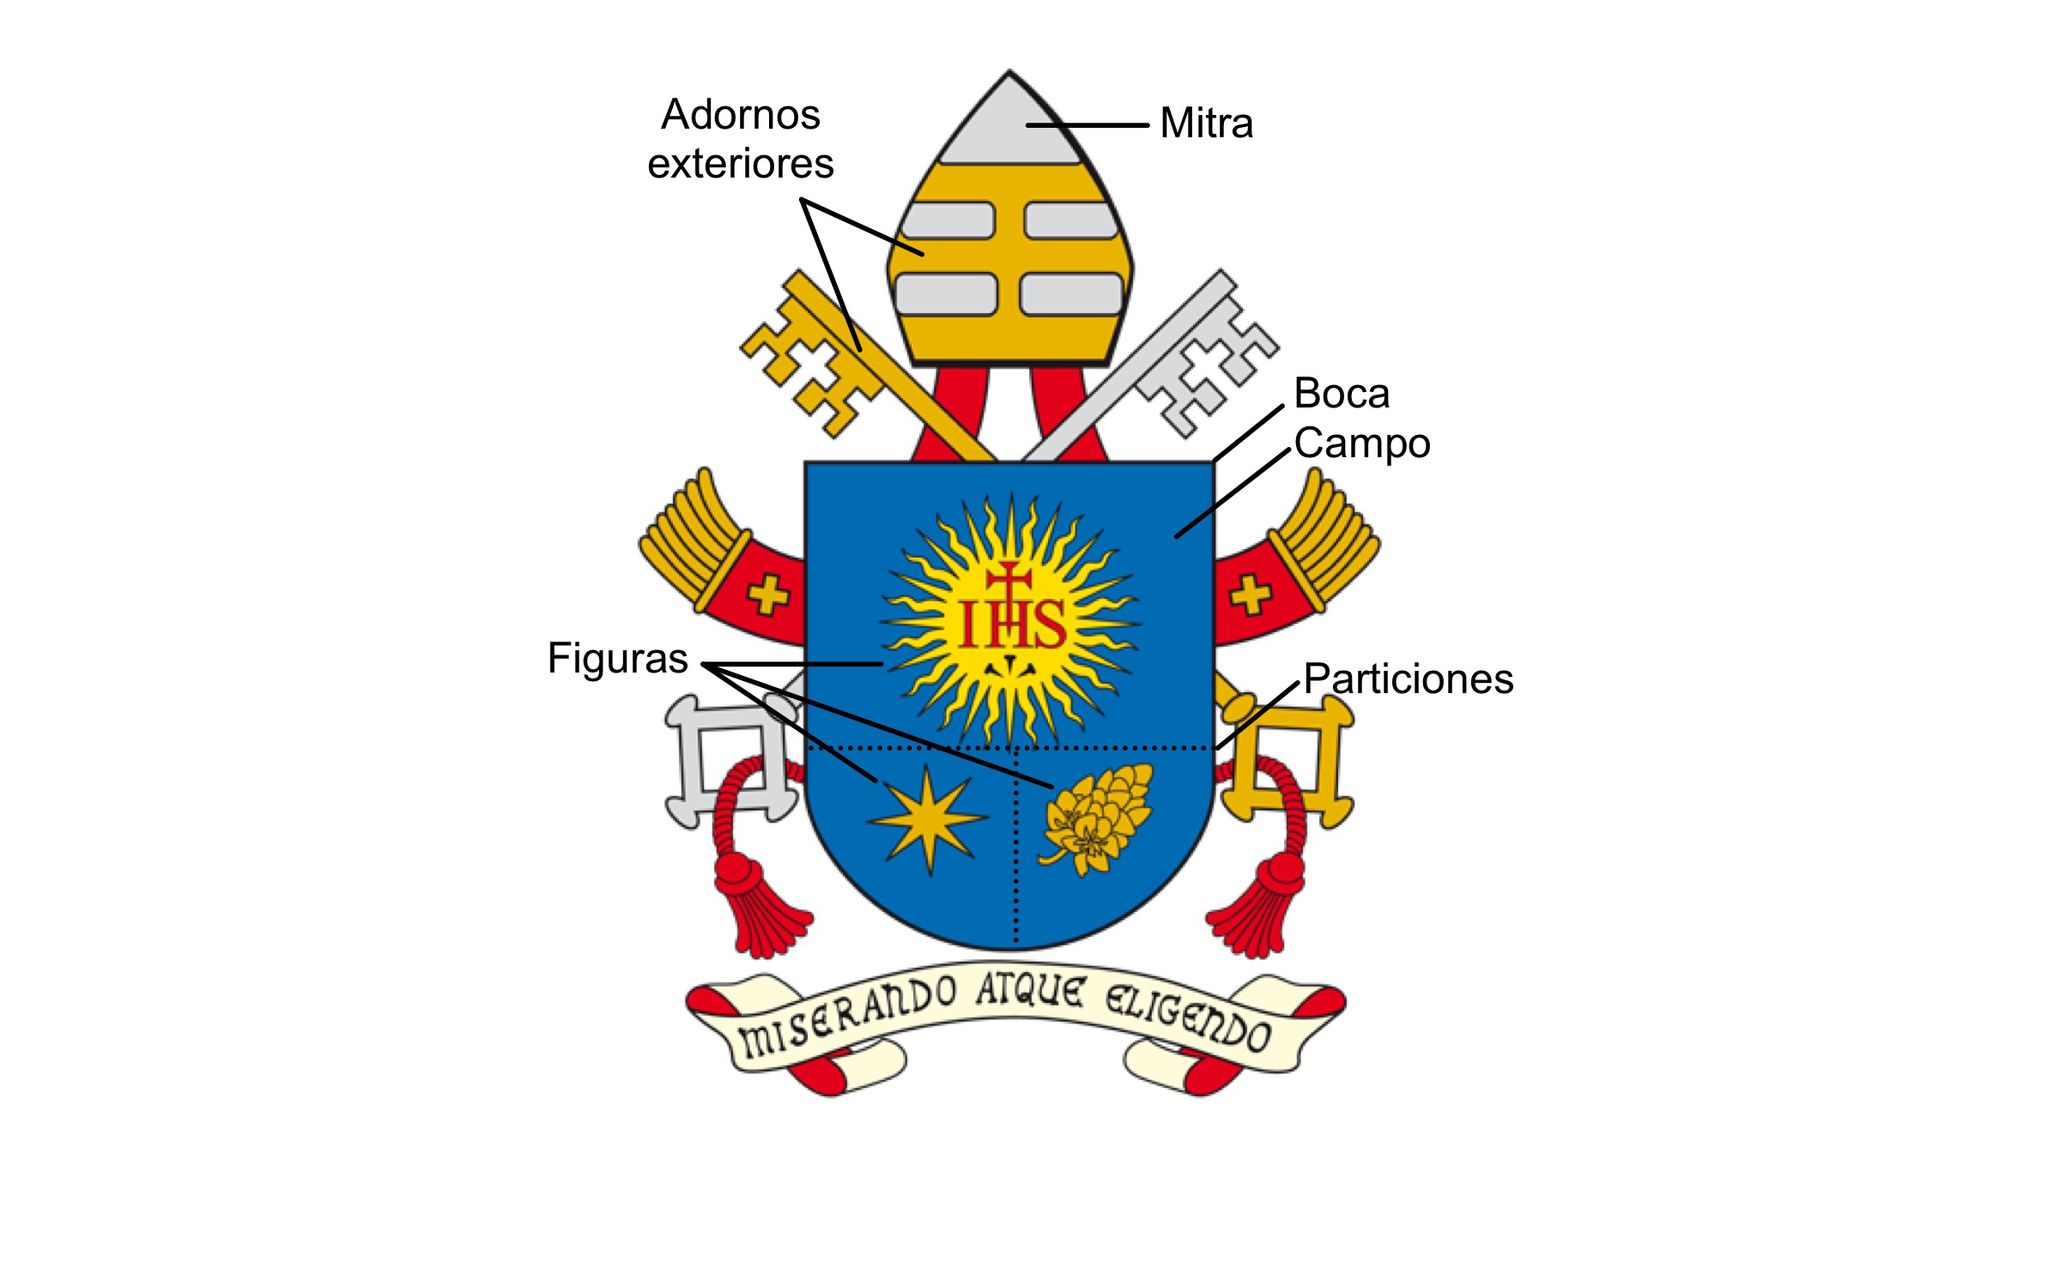
\includegraphics[width=0.9\textwidth]{figuras/escudo-papa-francisco.png}
    \caption{Escudo de armas del papa Francisco.}
\end{figure}

El desarrollo de esta considerada ciencia-arte, tiene sus raíces en la Europa medieval,
cuando la equipación militar hizo que fuese imposible identificar a simple vista a un 
caballero en combate, lo que los llevó a pintar símbolos en sus escudos. Con el tiempo,
estos símbolos fueron adquiriendo carácter hereditario y evolucionando hacia un sistema
de representación de linajes y alianzas. Paralelamente, en el siglo XIII surge la 
heráldica eclesiástica, adaptando este lenguaje gráfico a la jerarquía y simbología
de la Iglesia. Sobre los siglos XIV y XV, la heráldica se consolidó y comenzó a ser 
empleada como decoración en la arquitectura y como seña de identidad de instituciones, 
familias y territorios. \cite{messia1990,delgado2019,pierrerer1858}

Actualmente, la heráldica sigue siendo un campo de estudio relevante en disciplinas
como la historia y la historia del arte, pero presenta obstáculos que dificultan el 
acceso y la comprensión a quien desea introducirse a ella. La falta de una completa
digitalización y estandarización de esta disciplina, y la ausencia de tecnologías
actuales que faciliten su estudio, resulta en barreras para su aprendizaje, 
aplicación académica y divulgación.

Con la finalidad de hacer menos hostil el aprendizaje de esta ciencia-arte, este
proyecto busca desarrollar una herramienta que modernice y agilice el aprendizaje
de la heráldica, facilitando su comprensión y análisis, aspirando a ofrecer un 
recurso digital accesible que contribuya a la preservación y divulgación de esta 
disciplina.

Este proyecto es software libre, y está liberado con la licencia \cite{gplv3}.